\chapter{基础知识}
\label{chap:preliminary}

\textit{}

\textit{本章介绍本文研究所需的信息论、博弈论及隐私保护的基本概念,包括Shannon信息论及其扩展,策略博弈、扩展式博弈等博弈论概念,隐私分类及隐私保护基本模型。本章的内容主要为后文展开具体研究奠定基础。}
\section{Shannon信息论}

\subsection{信息通信模型}
信息论\cite{shannon1948mathematical,
	stone2018information}是信息科学的基本工具,信息论对于量化信息的不确定性和信息量有重要的作用。信息通信模型最早由Shannon在其《通信的数学原理》论文中提出,如图\ref{fig:communication-model}所示。

\begin{figure}[htbp]
	\centering
	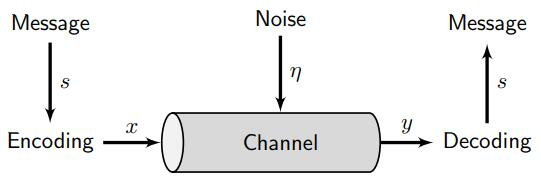
\includegraphics[width = 0.6\linewidth]{./figures/shannon-communicaiton-model.jpg}
	\caption{信息通信模型\cite{stone2018information}
	}
	\label{fig:communication-model}
\end{figure}

信息通信模型\cite{stone2018information}由信源消息、编码器、信道、解码器、信宿消息和噪音构成,信源消息(数据)在作为信道输入之前被编码器进行编码;编码后的信源消息在信道中传输,传输过程中会受到噪声影响;解码器从信道中接收到加噪后的信息,解码为信宿消息。Shannon定义的上述通信模型可以描述任何人造或自然的系统间的通信信息量。对任意额通信系统,都有:1)信道容量,即可以被信道传输信息的最大量;2)极限受损。即信道中最大的噪音量;3)通过编码,可以达到这两个极限。



\subsection{信息熵}


\begin{definition}
	对于事件集中的某一特定事件$x$,$x$的概率为$p(x)$,则$x$的香农信息为$-\text{log}p(x)$。
\end{definition}
上述定义通常被称为自信息,其表示该事件发生了所需要传递的信息的比特数量。自信息表示了事件所蕴含的信息量,自信息越大,该事件携带的信息量越多,反之越少。而熵表示自信息的平均量,即某一个随机事件变量的所有事件取值发生时,该随机变量的平均Shannon信息量,即

\begin{definition}
随机变量$X=(x_1,x_2,...,x_n)$,其概率分布为~$\{p(x_1),p(x_2),....,p(x_n)\}$~,则该随机变量的熵为
\begin{equation}
H(x)=-\sum_{i=1}^{n}p(x_i)log_2p(x_i)
\end{equation}
\end{definition}
在Shannon通信模型中,信源产生的随机事件的熵称为信源熵,信宿产生的随机事件的熵称为信宿熵。信源熵是信源消息变量~$X$~可以表示的平均信息比特数,即平均信息量。但是,上述定义给出的熵是离散变量的熵,对于连续熵的定义,本文不再讨论,可参考文献\cite{stone2018information}。

熵是对不确定度的一种度量,当不确定下降时,我们得到了信息,因此信息和熵是一体两面的。上述定义的熵是针对所有离散随机变量的,任意随机变量都存在一个概率分布,使得该随机变量的熵为最大,该分布称为最大熵分布。通过熵的定义可知,当$n$个随机事件均匀分布时,该随机变量熵最大,即有

\begin{equation}
H(x)_{Max}=-n\sum_{i=1}^{n}p(x_i)log_2p(1/n)
\end{equation}


针对Shannon通信模型,若在信源输入消息,则会对信宿消息的不确定度产生影响,从平均意义上就有平均不确定度的影响,即条件熵。

\begin{definition}
	随机变量$X=(x_1,x_2,...,x_n)$是输入,其概率分布为~$\{p(x_1),p(x_2),....,p(x_n)\}$~,随机变量$Y=(y_1,y_2,...,y_n)$是输出,其概率分布为~$\{p(y_1),p(y_2),....,p(y_m)\}$~,则输入$X$时,$Y$的不确定度为
	\begin{equation}
	H(Y/x)=-\sum_{i=1}^{n}-\sum_{j=1}^{m}p(y_j/x_i)log_2p(y_j/x_i)
	\end{equation}
\end{definition}


\subsection{互信息}

\begin{definition}
变量$X$与$Y$之间的互信息$I(X,Y)$是指,输入$X$时的每个随机事件能够提供给$Y$的平均信息量,互信息可以表示为
\begin{equation}
I(X,Y)=H(X)-H(X/Y)=H(Y)-H(Y/X)
\end{equation}
\end{definition}

互信息量描述了两个随机变量之间的信息量,可以认为是隐私保护前后,隐私分析前后,不同隐私信息变量间相差的隐私信息量。


%\subsection{结构信息论}

\section{博弈论}
博弈论\cite{owen2001game,gibbons1992game} 是一个自利参与者间相互作用的数学模型,用于为这些参与者寻找冲突与合作的解决方案。 博弈包含实体之间的迭代,并且每个博弈者在每次迭代中都将执行一个操作。 最后,博弈达到了解决方案(即平衡),所有博弈者都获得了自己最大的收益。 在特定的博弈中,博弈者是理性的,这意味着每个博弈者都会采取行动来响应他人的行动,以获取最大的利益。


\subsection{博弈模型}

一个博弈模型往往有三部分组成,1) 参与者集。博弈中往往包含一定数量的博弈参与者$N$;2)策略集合。每个参与者的可选策略集合。3)收益函数。每个用户在每次博弈过程中得到的可以量化的收益后损失。
对于每个参与者而言,由于其策略在博弈开始 的时候就定制好的,描述了每个参与者在任何情况下的执行行动,故其策略是复杂的。一些情况下,由于参与者的可选行动范围是非常小的,但也有时候执行行动的可选集合非常大,如象棋、围棋等,策略就变得异常复杂。

\subsection{策略博弈}
策略博弈是指博弈参与者仅进行一次博弈的博弈模型,根据不同的分类,策略博弈被定义为各种不同的策略博弈。

形式化地,策略博弈模型$\Gamma=(P,A,u)$中包含参与者$P=(P_1,P_2,...,P_n)$   、所有参与者行为集合$A=(A_1,A_2,...,A_n)$和效用函数$u=(u_1,u_2,...,u_n)$。称$n$个参与者的行为有序集合$a=(a_1,a_2,...,a_n)$为行为组态,其中$a_i \in A_i$是参与者$P_i$在其行为集合$A_i$中的一个策略选择。行为组态$a$可表示为$a=(a_i,a_{-i})$,其中$a_i$表示除参与者$P_i$之外参与者的策略组合。$u_i(a_i,a_{-i})$ 表示参与者$P_i$在策略组合$(a_i,a_{-i})$ 状态下的效用函数。

\begin{definition}
	在策略博弈模型中,对任意参与者$P_i \in P$,其效用函数有
	\begin{equation}
	u_i(a_i,a_{-i}) \geq 	u_i(a_i',a_{-i})
	\end{equation}
	其中$a_i'\in A_i$,则称策略组合$a=(a_1,a_2,...,a_n)$是该策略博弈的\textbf{Nash均衡}。
\end{definition}


\begin{definition}
	在策略博弈模型中,一个策略$a_i$是参与者$P_i$的\textbf{占优策略},当且仅当对于该参与者的其他任何策略$a_i'\neq a_i$和其他参与者可能的策略集合$a_{-i}$中,有
	
	\begin{equation}
	u_i(a_i,a_{-i}) \geq 	u_i(a_i',a_{-i})
	\end{equation}
\end{definition}

\begin{definition}
	当博弈模型中仅有两方参与者的时候,称之为\textit{二人博弈}。
\end{definition}

\begin{definition}
当博弈模型中仅有两方参与者的时候,称之为\textit{二人博弈}。
\end{definition}

\begin{definition}
二人博弈中,参与者1与参与者2分别有$n$种和$m$种可选策略,若参与者1选策略$i$,参与者2选策略~$j$~,其中~$i=1,2,...,n,j=1,2,...,m$~,则两个参与者进行博弈,且各自获取到了收益函数。若在一个博弈中,两方参与者一输一赢,且参与者1的收益是$u_{ij}$,参与者2的收益是$-u_{ij}$,则称该博弈是\textit{二人零和博弈}。
\end{definition}

\begin{definition}
	进一步地,若参与者1与参与者2各自的博弈收益之和是某个常数,则称该博弈是\textit{二人常和博弈}。
\end{definition}

当然,二人博弈的相关概念都可以扩展到多人,即\textit{$n$方博弈},\textit{$n$方零和博弈}与\textit{$n$方常和博弈}。博弈可分为合作博弈与非合作博弈,亦可分为完美信息博弈和非完美信息博弈。



\subsection{扩展式博弈}

扩展式博弈是策略博弈的一种扩展形式,该博弈模型可以描述参与者所有可能策略的序列,所有参与者在每次策略选择时所选策略,当参与者进行策略选择时对其他参与者策略选择的信息获取,所有策略选择组合对参与者自身的效用函数等不同的信息。扩展式博弈可以将参与者不完全信息表述为策略选择的自然可能性,即自然策略选择。

\begin{definition}
一般的,~$n$~个参与者的扩展式博弈包含以下信息:
\begin{enumerate}
	\item $n$个参与者有限集合$P=(p_1,p_2,...,p_n)$;
	\item 一颗有根博弈树;
	\item 博弈树的每个叶子节点有一个$n$元组效用函数,表示每个可能的博弈结果都对每个参与者都有一个收益。
	\item 博弈树的非叶子节点有一个含有$n+1$个自己的分割,该分割中一个子集是称为自然参与者的虚拟参与者,其余$n$个子集对应所有理性参与者。每个参与者子集中的节点是参与博弈的所有参与者。
	
	\item 自然参与者的每个节点的输出边上有一个概率分布;
	\item 每个理性参与者的每个节点集合被分割为信息集合,这些信息集合在参与者采取策略选择时,成为其不同的策略决策。
	\item 上述这些信息是每个理性参与者的公共常识。
\end{enumerate}
\end{definition}

类似地,扩展式博弈也可以划分为不同的子类,如完美信息博弈,非完美信息博弈,纯策略博弈,混合策略博弈,重复博弈,非重复博弈。扩展式博弈中有个重要的概念,即子博弈精炼纳什均衡,定义如下:
\begin{definition}
扩展式博弈的策略组合$a=(a_1,a_2,...,a_n)$是一个\textbf{子博弈精炼纳什均衡}当且仅当:如果它是原博弈的纳什均衡;它在每一个子博弈上也都构成纳什均衡。
\end{definition}
\subsection{演化博弈}

演化博弈将经典博弈中参与者的理性假设放宽为有限理性,并引入了群体演化.参与者的策略选择在每一次博弈中不一定是最优的,其可在演化过程中模仿其他参与者的高收益策略,调整其后续博弈策略以提高其收益。演化博弈关注所有参与者策略的动态平衡,其核心在于\textbf{演化稳定策略}。

\begin{definition}
	演化博弈中,若一个被所有个体采用的策略可成功抵抗所有其他策略的少量个体入侵,则此策略就被称为\textbf{演化稳定策略}。形式化地,若策略$a_e$满足
	\begin{equation}
	u(a_e,a_e) > u(a_i,a_e), \forall i \ne e 
	\end{equation}
	或
	\begin{equation}
	u(a_e,a_e) > u(a_i,a_e), \forall i \ne e,\\
	u(a_e,a_i) > u(a_i,a_i), \forall i \ne e 
	\end{equation}
	则称策略$a_e$为演化稳定策略,其中$u(a_e,a_i)$表示当策略$a_e$遇到$a_i$时, $a_e$的收益。
	
\end{definition}


\section{隐私定义及隐私保护}
隐私是一种社会化的概念,最早认为是一种不被打扰的权利,随着数据应用的越来越广泛,场景越来越复杂多样,隐私逐步转变为一种形式化,可量化的概念,需要学术界进行深入研究,以便在数字社会时代更好的理解隐私,更好的保护隐私,更好的应用数据。

\begin{definition}
	隐私是个体或群体隐藏自己身份、有关自己信息,进而有选择性的表达自己的能力。
\end{definition}

上述定义来自Wiki百科,是一种描述性的定义。不同文化背景,不同社会阶层的不同个体,对隐私的边界和内容都不尽一致。不过由此,可以将隐私分为三类,即身份隐私、属性隐私和隐私表达。

\subsection{身份隐私}
\begin{definition}
身份隐私是个体或群体隐藏自己身份的能力。
\end{definition}

在数字中时代,包含大量个人信息的数据被广泛的存储在云端、智能终端、各类应用中,身份隐私就变为在一个数据集中、一个通信系统中个人隐藏自己唯一标识、伪标识信息的能力。可以将身份隐私细分为两类隐私,第一类匿名隐私,即在一个特定群体里,无法区别某个特定个体的身份;第二类关系隐私,即判别一个特定个体是否属于某一个特定群体。
\begin{definition}
	匿名隐私是个体隐藏自己在一个群体里无法被唯一区别出来的能力。
\end{definition}

匿名隐私蕴含着一个背景知识,即已知该个体属于该群体,需要保护其身份。例如需要保护住院病人群体中病人的身份,以保护其不被区别出来是哪一个病人。在基于位置服务、社交网络、基因数据等各类场景中都存在匿名隐私,也需要保护匿名隐私。因此,不同类型的匿名性被形式化定义并扩展,如~$k$~匿名\cite{sweeney2002k}、~$l$~多样性匿名\cite{machanavajjhala2007l}、~$t$~邻近匿名\cite{li2007t}等,特别注意的是匿名性的定义伴随着隐私的量化,即上述匿名隐私中的\textit{能力}的量化。

\begin{definition}
	关系隐私是个体隐藏自己被判断是否属于某一个特定群体成员的能力。
\end{definition}

关系隐私是要求比匿名隐私更强的隐私,即其去掉了匿名隐私中的背景知识假设,对隐私保护的要求更高。某特定的人需要隐藏自己,不让敌手判断出其是否属于住院群体中的一员;莫人也需要保护自己,不让敌手知道自己是否属于某个社交群体。关系隐私还可分类为积极关系隐私和消极关系隐私。
\begin{definition}
	积极关系隐私是个体隐藏自己被判断属于某一个特定群体成员的能力。
\end{definition}

\begin{definition}
	关系隐私是个体隐藏自己被判断不属于某一个特定群体成员的能力。
\end{definition}

\subsection{属性隐私}
属性隐私是一种比匿名隐私假设更弱的隐私要求,即某特定的个体已经被唯一识别出来,需要保护其个人信息,如身高、爱好、政治倾向、疾病状况、疾病易感特性等。

\begin{definition}
	属性隐私是个体或群体隐藏自己信息的能力。
\end{definition}

属性隐私的场景最复杂,也最多样化,不同个体对隐私边界即隐私内容的界定也往往区别于此。正是如此,属性隐私需要更多的、更深入的研究,以提供更加个性化、更加自适应、更加全面的隐私保护。

\subsection{隐私表达}

\begin{definition}
	隐私表达是个体或群体表达自己身份隐私或属性隐私的能力。
\end{definition}

隐私表达是一种更高的要求,是在保障个人身份隐私和属性隐私的基础上,能够自主可控的表达个人隐私的能力。

目前,对匿名隐私的研究较多,关系隐私的研究和属性隐私的研究次之,对隐私表达的研究较少,除了更加具体的形式化表达不同场景下的不同隐私,即形成了隐私的形式化定义,对隐私形式化定义的基础上需要可量化、可比较的方法,即形成了隐私度量。这些领域都需要进一步研究。

\subsection{隐私保护模型}

对上述三类隐私定义的实现方法需求,产生了隐私保护机制的研究,如实现~$k$~匿名性的算法\cite{sweeney2002k}实现差分隐私定义的差分隐私算法\cite{dwork2006differential},一般的隐私保护模型如图\cite{cha1-ppm.jpg}所示。

\begin{figure}[htbp]
	\centering
	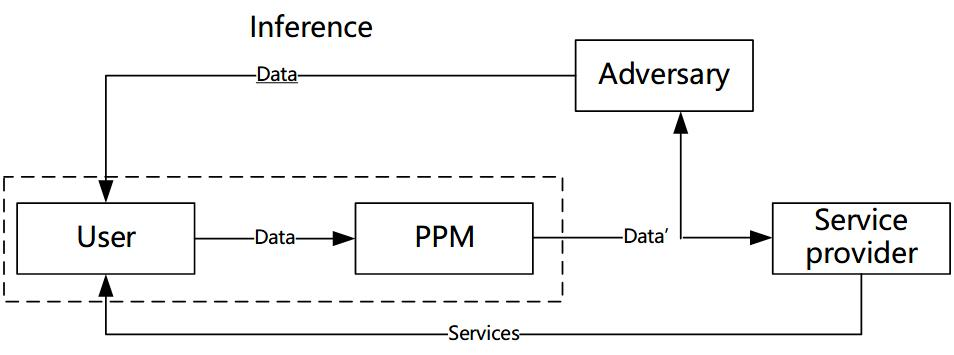
\includegraphics[width = 0.6\linewidth]{./figures/cha1-ppm.jpg}
	\caption{隐私保护模型}
	\label{fig:ppm-model}
\end{figure}

包含用户个人信息的隐私数据通过一定的隐私保护机制进行保护,提交给服务提供者并从其获得数据服务,在此过程中会受到不同能力的敌手的隐私分析。

关于隐私保护机制,针对不同的隐私定义和隐私目标,不同的隐私保护算法被设计出来,形成了\textit{隐私保护算法研究};同时对因保护机制的能力量化形成了隐私保护机制评价研究,即\textit{隐私保护能力度量};在敌手针对隐私进行分析的过程中,设计了不同的隐私分析算法,即形成了\textit{隐私分析研究};同样,对隐私分析能力也需要度量,量化被攻击者的隐私损失,量化敌手的隐私获取量等,即\textit{隐私分析能力度量研究};数据共享应用的目的是获得较好的数据服务,即数据效用,但隐私保护需求和数据效用需求相互冲突,又相互依赖,需要平衡二者的关系,即产生了\textit{理性隐私保护研究};在理性隐私保护领域,隐私和效用往往需要能够统一的量化、比较和交换,又进一步产生了\textit{隐私效用度量研究}。

\section{小结}

本章简要介绍了信息论、博弈论和隐私保护模型的基本知识,其中信息论作为本文的基础性工具,在后续的每一部分都将使用相关概念和方法,以对隐私定义并量化,对隐私保护能力度量和评价,对隐私分析能力进行度量和评价;博弈论作为主要的工具帮助本文在后续章节实现理性的隐私保护方案设计,以动态的、自适应的实现数据隐私保护和数据效用间的平衡;隐私保护模型是本文研究的核心基础,本文的所有研究都围绕该模型展开,包括统一的隐私度量框架、序列型数据属性隐私分析与量化、面向隐私保护的风险自适应访问控制隐私保护和理性隐私风险访问控制模型。